\section{Tableros de Control y Analítica (Dashboards)}

Este manual ha sido diseñado para explicar de manera sencilla y clara qué información muestra cada tablero (dashboard) del sistema, de dónde proviene esa información y para qué sirve. Está pensado para que cualquier persona del equipo pueda entender la salud del negocio de un vistazo.

\subsection{Tablero de Ventas (Sales)}
Este tablero es el centro principal para evaluar el desempeño comercial de la empresa. La información se actualiza dinámicamente y puede ser filtrada por distintos periodos de tiempo (por defecto "Últimos 90 días").

\textbf{¿De dónde se extrae la información general?}\\
Toda la data de esta pantalla proviene del módulo de \textbf{Ventas} de Odoo. Se alimenta automáticamente de los presupuestos (Cotizaciones) y de las ventas confirmadas (Órdenes de Venta) gestionadas por el equipo comercial.

\subsubsection*{Análisis de las métricas y gráficos disponibles:}
\begin{itemize}[leftmargin=*]
    \item \textbf{Tarjetas de Indicadores Principales (KPIs superiores):}
    \begin{itemize}
        \item \textbf{Cotizaciones:} Total de presupuestos generados y enviados a los clientes que aún no se han cerrado.
        \item \textbf{Confirmados:} Número total de ventas que ya han sido aceptadas y oficializadas.
        \item \textbf{Ingreso:} Monto total de dinero generado por las ventas confirmadas en el periodo seleccionado.
        \item \textbf{Orden promedio:} El valor monetario promedio de cada venta (Ingresos divididos entre las Órdenes confirmadas). Ayuda a entender el nivel de gasto habitual de los clientes.
    \end{itemize}
    \item \textbf{Gráfico ``Ventas mensuales'' (Monthly Sales):}
    \begin{itemize}
        \item Muestra la evolución de los ingresos a lo largo del tiempo. Es fundamental para identificar patrones estacionales (meses de alta o baja demanda en turismo).
    \end{itemize}
\end{itemize}

\subsubsection*{Tablas de Ranking y Desempeño:}
Estas secciones organizan la información de mayor a menor para identificar rápidamente las mejores oportunidades comerciales.

\begin{itemize}[leftmargin=*]
    \item \textbf{Top Quotations (Mejores cotizaciones) y Top Sales Orders (Órdenes de venta principales):}
    \begin{itemize}
        \item Muestran lasTableros de Control y Analítica (Dashboards) negociaciones de mayor valor económico. Detallan el Cliente, el Vendedor a cargo y el monto potencial o cerrado (Revenue).
        \item \textit{Fuente:} Cotizaciones pendientes y Órdenes de venta confirmadas, respectivamente.
    \end{itemize}
    \item \textbf{Top Products (Productos más vendidos) y Categorías:}
    \begin{itemize}
        \item Identifican qué tours específicos y qué familias de productos (ej. "Packages", "Inca Trail") están generando más ingresos y mayor volumen de pedidos.
        \item \textit{Fuente:} Las líneas de detalle (los tours específicos agregados) dentro de cada Orden de Venta.
    \end{itemize}
    \item \textbf{Top Countries (Mejores países) y Top Customers (Mejores clientes):}
    \begin{itemize}
        \item Permiten visualizar geográficamente de dónde provienen los compradores y revelar quiénes son los clientes individuales que más invierten.
        \item \textit{Fuente:} La información de perfil y dirección del contacto asociado a la Orden de Venta.
    \end{itemize}
    \item \textbf{Top Sales Teams (Equipos) y Top Salespeople (Vendedores):}
    \begin{itemize}
        \item Evalúa el rendimiento del personal interno, mostrando qué equipo y qué asesor de ventas está cerrando más tratos y atrayendo mayor cantidad de dinero.
        \item \textit{Fuente:} El campo "Vendedor" y "Equipo de Ventas" asignado a cada venta.
    \end{itemize}
    \item \textbf{Top Sources (Orígenes) y Top Mediums (Medios de adquisición):}
    \begin{itemize}
        \item Analizan por qué canal publicitario o vía de contacto llegó la venta (ej. referidos, sitio web, redes sociales). Es vital para evaluar la efectividad del área de marketing.
        \item \textit{Fuente:} Las etiquetas de rastreo (UTM) registradas en Odoo al momento en que el prospecto inició el contacto.
    \end{itemize}
\end{itemize}

\begin{figure}[h!]
    \centering
    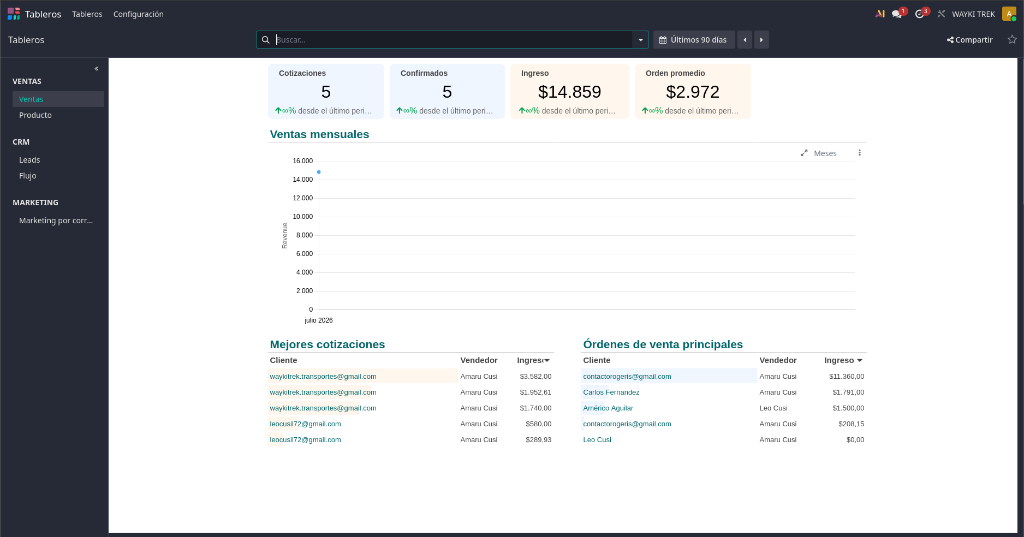
\includegraphics[width=0.9\textwidth]{assets/tablero_5_sales.png}
    \caption{Tablero de Ventas}
\end{figure}

\clearpage

\subsection{Tablero de Productos (Product)}
Este tablero está enfocado enteramente en analizar \textit{qué} es lo que se está vendiendo (qué tours, servicios o paquetes generan más interés y rentabilidad), dejando en un segundo plano las métricas generales de dinero de la empresa.

\textbf{¿De dónde se extrae la información general?}\\
Se nutre de la combinación del catálogo de \textbf{Productos} y el módulo de \textbf{Ventas}. El sistema desglosa y analiza cada línea de detalle dentro de las facturas y órdenes de venta confirmadas para saber exactamente qué servicio específico se compró.

\subsubsection*{Análisis de las métricas y gráficos disponibles:}
\begin{itemize}[leftmargin=*]
    \item \textbf{Tarjetas de Indicadores Principales (KPIs superiores):}
    \begin{itemize}
        \item \textbf{Más vendido:} Muestra el producto o tour exacto que ha tenido más éxito en volumen durante el periodo evaluado.
        \item \textbf{Mejor categoría:} Identifica cuál familia de servicios (ej. "Packages", "Inca Trail") es la favorita absoluta de los clientes en general.
    \end{itemize}
    \item \textbf{Gráficos de Barras de Desempeño:}
    \begin{itemize}
        \item \textbf{Best Sellers by Revenue (Mejores productos por ingresos):} Muestra de forma visual qué productos específicos están dejando la mayor cantidad neta de dinero a la empresa. Sirve para entender qué servicios son los más rentables.
        \item \textbf{Best Sellers by Units Sold (Mejores productos por volumen):} Muestra qué productos tienen la mayor rotación o salida (independientemente de si son baratos o caros). Es vital para saber qué tours atraen a la mayor masa de turistas.
    \end{itemize}
\end{itemize}

\subsubsection*{Tablas de Ranking y Detalle:}
\begin{itemize}[leftmargin=*]
    \item \textbf{Best Selling Products (Productos más vendidos):}
    \begin{itemize}
        \item Una tabla exhaustiva que clasifica todo el catálogo ofertado. Por cada tour o servicio, detalla exactamente cuántas unidades/pasajes se vendieron (Units) y cuánto dinero exacto generaron (Revenue).
        \item \textit{Fuente:} El recuento total de los artículos facturados en las ventas ganadas.
    \end{itemize}
    \item \textbf{Category (Rendimiento por Categoría):}
    \begin{itemize}
        \item En lugar de analizar producto por producto, esta tabla agrupa las ventas por familias enteras. Permite a la gerencia decidir qué macro-categorías de viaje vale la pena potenciar en futuras campañas.
        \item \textit{Fuente:} El campo "Categoría de Producto" configurado en el inventario de Odoo.
    \end{itemize}
\end{itemize}

\begin{figure}[h!]
    \centering
    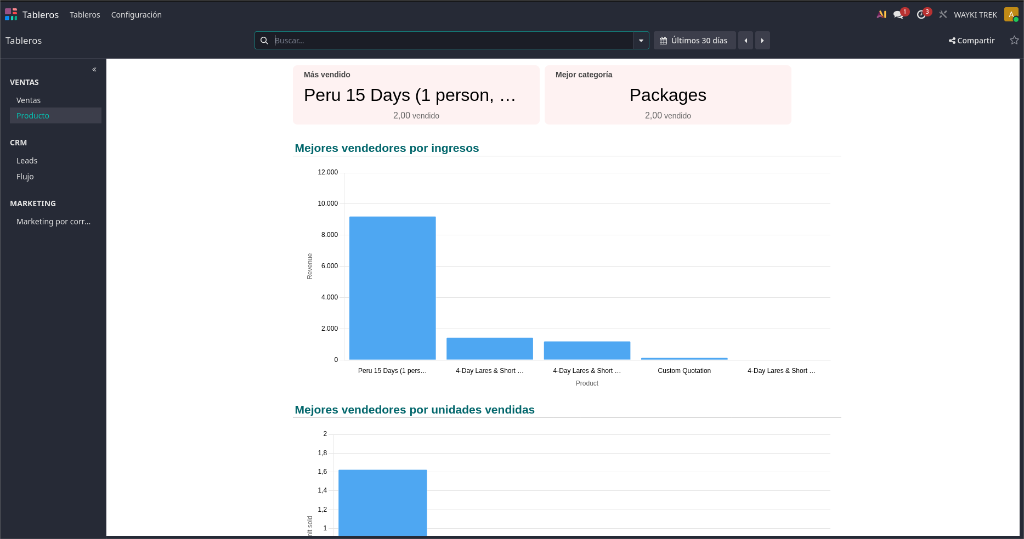
\includegraphics[width=0.9\textwidth]{assets/tablero_6_product.png}
    \caption{Tablero de Productos}
\end{figure}

\clearpage

\subsection{Tablero de Leads (Prospectos)}
Un "Lead" o prospecto es una persona o contacto que ha mostrado interés en nuestros servicios (por ejemplo, llenando un formulario en la página web o mandando un correo), pero que todavía no ha recibido una cotización formal. Este tablero evalúa cómo atraemos y gestionamos a esos posibles clientes.

\textbf{¿De dónde se extrae la información general?}\\
Toda la información fluye desde el módulo de \textbf{CRM} (Gestión de Relaciones con el Cliente). Se alimenta automáticamente cada vez que ingresa una nueva consulta al sistema y se registra como una oportunidad de venta inicial.

\subsubsection*{Análisis de las métricas y gráficos disponibles:}
\begin{itemize}[leftmargin=*]
    \item \textbf{Tarjetas de Indicadores Principales (KPIs superiores):}
    \begin{itemize}
        \item \textbf{Índice de acuerdos (Win Rate):} Muestra qué porcentaje histórico de prospectos termina convirtiéndose en clientes reales. Es la medida clave del éxito de las ventas.
        \item \textbf{Tamaño promedio de trato:} Cuánto dinero se espera ganar, en promedio, por cada prospecto nuevo que ingresa al sistema.
        \item \textbf{Ingreso:} El dinero total real que ha ingresado a partir de los prospectos generados en este periodo.
        \item \textbf{Días para ganar / Días hasta asignar:} Miden la agilidad del equipo. Cuánto tiempo pasa desde que un prospecto nos contacta hasta que un vendedor lo atiende, y cuántos días pasan hasta que finalmente paga.
    \end{itemize}
    \item \textbf{Gráfico ``Leads por mes'' (Leads by Month):}
    \begin{itemize}
        \item Visualiza el volumen de consultas que llegan mes a mes. Es fundamental para saber en qué épocas del año la empresa recibe más correos y solicitudes de información.
    \end{itemize}
\end{itemize}

\subsubsection*{Tablas de Ranking y Segmentación:}
\begin{itemize}[leftmargin=*]
    \item \textbf{Top Countries (Mapa y Países principales):}
    \begin{itemize}
        \item Un mapa mundial y una tabla que muestran visualmente de qué países provienen las personas que nos contactan. Es información vital para la gerencia al decidir en qué territorios invertir dinero para publicidad (ej. pautas en Google o Facebook).
        \item \textit{Fuente:} El país registrado por el cliente en el formulario web o en su perfil de contacto.
    \end{itemize}
    \item \textbf{Top Tags (Etiquetas principales) y Top Lost Reasons (Motivos de pérdida):}
    \begin{itemize}
        \item Identifican qué tipo de intereses tienen los prospectos (usando etiquetas como "Aventura", "VIP") y, lo más crítico, \textbf{por qué se pierden las ventas} (ej. "Precio alto", "Falta de cupos").
        \item \textit{Fuente:} Las etiquetas agregadas por los vendedores y el "Motivo de pérdida" que seleccionan al descartar una oportunidad en el CRM.
    \end{itemize}
    \item \textbf{Top Campaigns, Sources y Mediums (Campañas, Orígenes y Medios):}
    \begin{itemize}
        \item Estas tres tablas analizan exactamente qué campaña publicitaria, buscador o red social está atrayendo a la mayor cantidad de prospectos, y cuáles traen a los prospectos más rentables.
        \item \textit{Fuente:} Los enlaces de rastreo de marketing (UTM) que Odoo captura de forma invisible cuando el cliente hace clic en un anuncio antes de llenar el formulario web.
    \end{itemize}
    \item \textbf{Top Sales Teams y Top Salespeople (Equipos y Vendedores):}
    \begin{itemize}
        \item Mide qué miembro del equipo y qué grupo de ventas están recibiendo y procesando la mayor cantidad de consultas nuevas, y cuántos ingresos logran materializar a partir de ellas.
        \item \textit{Fuente:} El vendedor asignado de forma automática o manual al Lead dentro del CRM.
    \end{itemize}
\end{itemize}

\begin{figure}[h!]
    \centering
    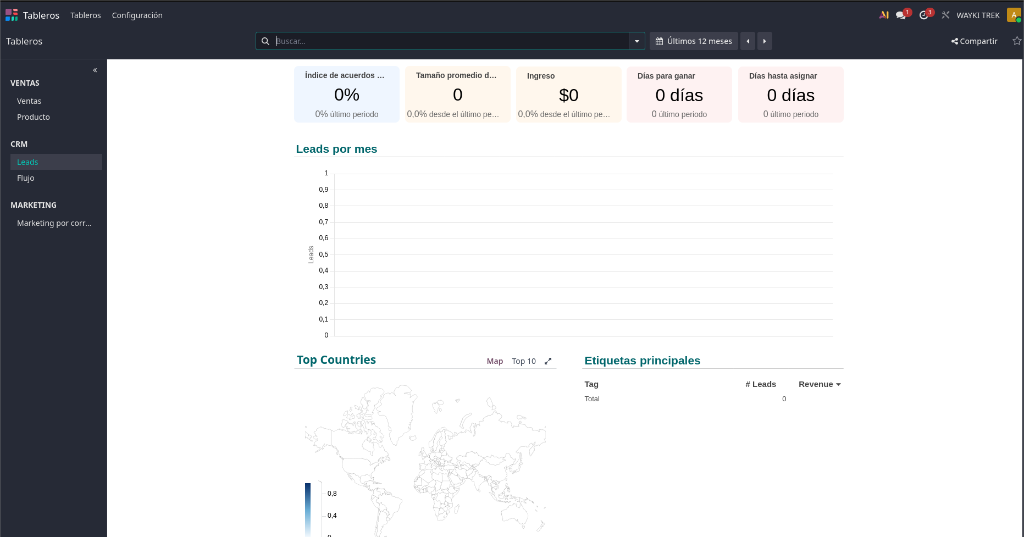
\includegraphics[width=0.9\textwidth]{assets/tablero_1_leads.png}
    \caption{Tablero de Leads}
\end{figure}

\clearpage

\subsection{Tablero de Flujo (Pipeline)}
El "Pipeline" o embudo de ventas representa el proceso paso a paso por el que pasa un cliente potencial: desde el inicio de la negociación hasta que finalmente reserva y paga el tour. A diferencia del tablero de Leads, aquí nos enfocamos en el valor monetario que está "sobre la mesa" y a punto de ganarse.

\textbf{¿De dónde se extrae la información general?}\\
Al igual que los Leads, se extrae del módulo de \textbf{CRM}, pero aquí la información se filtra y se enfoca exclusivamente en las "Oportunidades" (personas que ya pasaron el primer filtro y están en un proceso de negociación serio con los vendedores).

\subsubsection*{Análisis de las métricas y gráficos disponibles:}
\begin{itemize}[leftmargin=*]
    \item \textbf{Tarjetas de Indicadores Principales (KPIs superiores):}
    \begin{itemize}
        \item \textbf{Esperado:} Es una proyección financiera. Suma el dinero total que ingresaría a la empresa si los vendedores logran cerrar con éxito todas las negociaciones activas.
        \item \textbf{Cerrado:} El dinero real que ya se ganó definitivamente y se cerró en el periodo evaluado.
        \item \textbf{Oportunidades abiertas:} El número exacto de negociaciones en curso que los vendedores están atendiendo activamente hoy.
    \end{itemize}
    \item \textbf{Gráficos de Progreso y Tiempo:}
    \begin{itemize}
        \item \textbf{Pipeline (Embudo por Etapa):} Muestra visualmente dónde se encuentran agrupados los clientes. Sirve para detectar "cuellos de botella" (por ejemplo, si el sistema alerta que hay 50 personas estancadas en la etapa "Cotización enviada" que no han avanzado).
        \item \textbf{Cierre esperado (Expected Closing):} Un gráfico que proyecta en qué fechas futuras ingresará el dinero a la empresa, basándose en la "Fecha límite" estimada que el vendedor le asigna a cada negociación en el CRM.
    \end{itemize}
\end{itemize}

\subsubsection*{Tablas de Ranking y Análisis Estratégico:}
\begin{itemize}[leftmargin=*]
    \item \textbf{Top Opportunities (Mejores oportunidades):}
    \begin{itemize}
        \item Es posiblemente la tabla más crítica para la gerencia. Enlista las negociaciones individuales de mayor valor económico. Detalla la Oportunidad, la Etapa actual, el Vendedor responsable, el País, el monto de dinero potencial (Revenue) y el Porcentaje de Éxito (Success \%) estimado.
        \item \textit{Fuente:} El listado directo de Oportunidades activas en el tablero Kanban del CRM.
    \end{itemize}
    \item \textbf{Desglose Geográfico (Country y Top Cities):}
    \begin{itemize}
        \item Tablas que agrupan el valor de las negociaciones activas según el país o la ciudad específica del prospecto. Útil para lanzar ofertas dirigidas a ciudades específicas.
        \item \textit{Fuente:} La ciudad y país registrados en la ficha de contacto del CRM.
    \end{itemize}
    \item \textbf{Orígenes y Medios (Top Sources y Top Mediums):}
    \begin{itemize}
        \item Indican por qué vía (ej. buscador de Google) y medio (ej. campaña de Facebook Ads) llegaron los clientes con los que se está negociando el dinero actualmente.
        \item \textit{Fuente:} Las etiquetas de rastreo (UTM) que acompañan al prospecto desde su primer clic en internet.
    \end{itemize}
    \item \textbf{Desempeño Interno (Top Salespeople y Top Sales Teams):}
    \begin{itemize}
        \item A diferencia del tablero de Ventas (que mide victorias finales), estas tablas evalúan el potencial en curso. Muestran qué vendedor y qué equipo tienen la mayor carga de negociaciones abiertas y la mayor suma de dinero proyectado. Ayuda a redistribuir el trabajo si alguien está sobrecargado.
        \item \textit{Fuente:} El responsable asignado en la ficha de la Oportunidad dentro del CRM.
    \end{itemize}
\end{itemize}

\begin{figure}[h!]
    \centering
    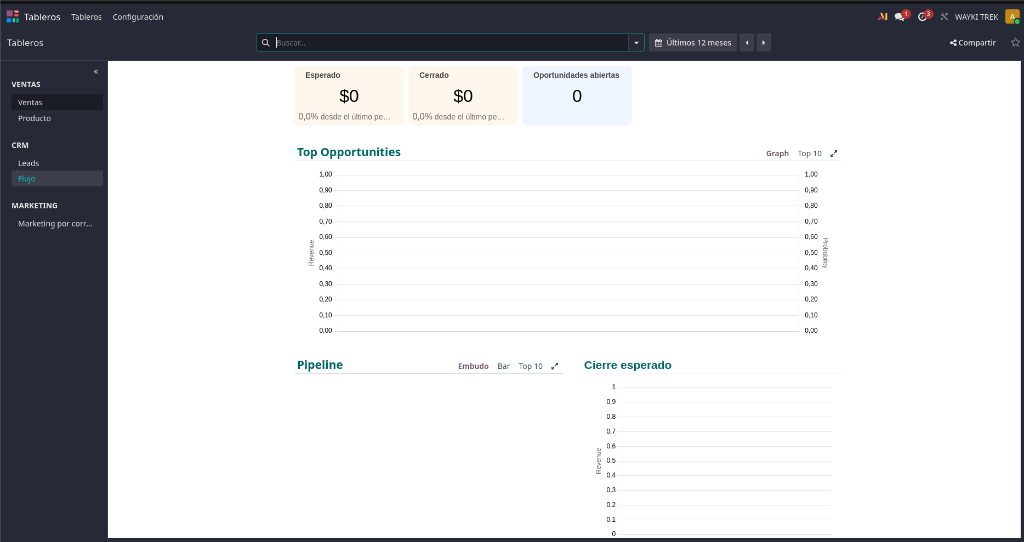
\includegraphics[width=0.9\textwidth]{assets/tablero_2_pipeline.png}
    \caption{Tablero de Flujo}
\end{figure}

\clearpage

\subsection{Tablero de Marketing por Correo (Email Marketing)}
Este tablero mide exclusivamente el impacto y éxito de las campañas masivas, boletines informativos (newsletters) o automatizaciones enviadas por correo electrónico a la base de datos de la empresa.

\textbf{¿De dónde se extrae la información general?}\\
Directamente del módulo de \textbf{Marketing por Correo (Email Marketing)}. Odoo inserta de forma automática rastreadores invisibles (píxeles) y enlaces trackeables en cada correo saliente, lo que le permite saber exactamente qué hace el cliente después de recibir el mensaje.

\subsubsection*{Análisis de las métricas y gráficos disponibles:}
\begin{itemize}[leftmargin=*]
    \item \textbf{Tarjetas de Indicadores Principales (KPIs superiores):}
    \begin{itemize}
        \item \textbf{Enviados / Abiertos:} Volumen total de correos que salieron del servidor y cuántos de ellos fueron realmente abiertos por el destinatario.
        \item \textbf{Tasa de entrega / Tasa de devolución (Bounced):} Indica la salud de la base de datos. Una alta tasa de devolución significa que muchos correos de tus contactos están mal escritos o ya no existen.
        \item \textbf{Tasa de abiertos / Tasa de clics (CTR):} Miden el nivel de interés. Una alta tasa de abiertos indica que el "Asunto" del correo fue muy atractivo. Una alta tasa de clics indica que el contenido interno (ofertas, botones) fue convincente.
        \item \textbf{Canceló su suscripción:} El porcentaje de personas que se aburrieron y decidieron darse de baja de la lista.
    \end{itemize}
    \item \textbf{Gráficos de Tendencia (Mails sent per month / Over previous period):}
    \begin{itemize}
        \item Gráficos de barras apiladas que comparan el volumen de correos enviados mes a mes (o frente al mes pasado). Clasifican visualmente qué porción de esos envíos fue Entregada, Respondida, Abierta o Cancelada.
    \end{itemize}
\end{itemize}

\subsubsection*{Tablas de Ranking y Monitoreo de Campañas:}
\begin{itemize}[leftmargin=*]
    \item \textbf{Top 10 recent mailing campaigns (Top 10 campañas recientes):}
    \begin{itemize}
        \item Una radiografía exacta de los últimos correos masivos enviados. Muestra el Asunto, la fecha exacta y un desglose estadístico profundo (en porcentajes y números totales) de cuántos lo recibieron, lo abrieron, lo respondieron o hicieron clic adentro.
        \item \textit{Fuente:} El registro estadístico de la aplicación de Email Marketing.
    \end{itemize}
    \item \textbf{Mailing campaigns in preparation (Campañas en preparación):}
    \begin{itemize}
        \item Funciona como una sala de espera operativa. Muestra los correos que están redactados en estado "Borrador" (ej. "Promociones para Mayo", "Recordatorio de cumpleaños"), quién es el vendedor responsable de enviarlos y a qué modelo de contactos (ej. lista de correo, lead o cliente) van dirigidos.
    \end{itemize}
    \item \textbf{Top 10 best link trackers (Top 10 enlaces más clickeados):}
    \begin{itemize}
        \item Evalúa qué botones o enlaces específicos dentro de tus correos llamaron más la atención. Detalla el título del enlace, hacia qué URL objetivo o WhatsApp dirigía (ej. "https://wa.me/...") y el número total de clics que recibió.
        \item \textit{Fuente:} El motor de rastreo de enlaces (Link Tracker) que Odoo incrusta al construir las plantillas de correo.
    \end{itemize}
\end{itemize}

\begin{figure}[h!]
    \centering
    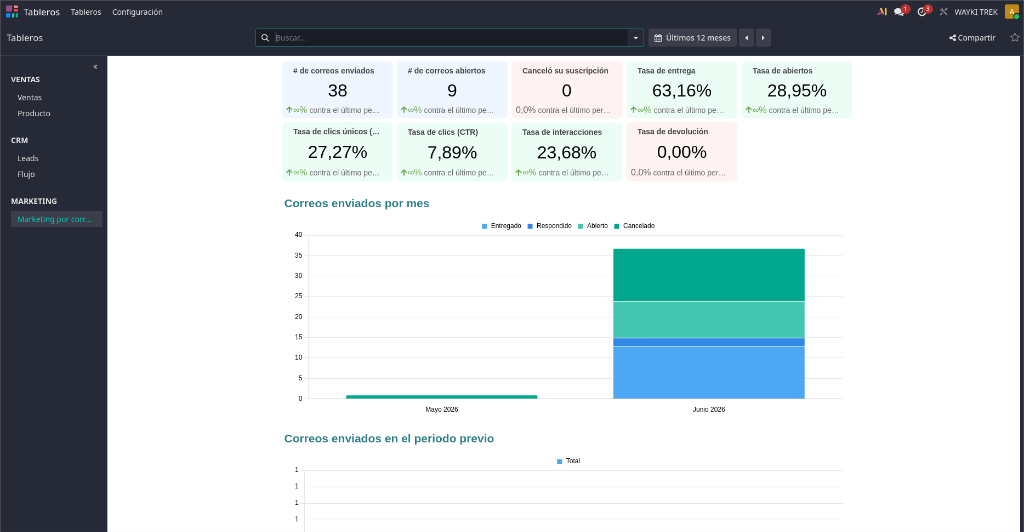
\includegraphics[width=0.9\textwidth]{assets/tablero_3_email_marketing.png}
    \caption{Tablero de Marketing por Correo}
\end{figure}
